\documentclass[12pt]{article}
\usepackage[margin=1in]{geometry}
\usepackage{hyperref}
\usepackage{graphicx}
\usepackage{booktabs}
\usepackage{setspace}
\usepackage{parskip}
\onehalfspacing
 
\title{Problem Set 6: Data Cleaning\\
       \large 2024 MLB Home Run Leaders\\
       \normalsize Source: MLB Stats API}
\author{Emilian Zavala}
\date{\today}
 
\begin{document}
\maketitle

\section{Data Source}
 
The data used in this problem set are the 2024 MLB Home Run Leaders pulled directly from the MLB Stats API. The endpoint used was:
 
\begin{center}
\small\texttt{https://statsapi.mlb.com/api/v1/stats/leaders?leaderCategories=homeRuns\&season=2024\&limit=50}
\end{center}
 
This returns a JSON object containing the top 50 home run leaders for the 2024 regular season, including each player's rank, full name, player ID, team name, and home run total. The data were parsed in R using the \texttt{rjson} package and flattened into a data frame using \texttt{sapply()}, identical to the approach used in Problem Set 5.

\section{Cleaning and Transformation Steps}
 
\subsection{Fixing Data Types}
 
When the JSON response is parsed and flattened into a data frame, all values arrive as character strings. The \texttt{Rank} and
\texttt{Home\_Runs} columns were explicitly converted to integers using \texttt{as.integer()} so that numeric operations and visualizations work correctly.
 
\subsection{Checking for Missing Values}
 
A column-wise missing value check using \texttt{colSums(is.na())} confirmed that the API returned complete data with no missing values across any variable. This is expected given that the endpoint only returns players with a recorded home run total.
 
\subsection{Cleaning Player and Team Names}
 
Player names and team names were passed through \texttt{stringr::str\_trim()} to remove any leading or trailing whitespace that may have been introduced during JSON parsing.
 
\subsection{Splitting Player Names}
 
The \texttt{Player} column contains each player's full name as a single string. For additional flexibility in analysis, the full name was split into separate \texttt{First\_Name} and \texttt{Last\_Name} columns using \texttt{stringr::word()}.
 
\subsection{HR Tier Classification}
 
A categorical variable \texttt{HR\_Tier} was created to group players into four performance tiers based on their home run total:
 
\begin{itemize}
  \item \textbf{Elite (45+)} --- historically exceptional power output
  \item \textbf{Great (35--44)} --- All-Star caliber power
  \item \textbf{Above Average (25--34)} --- solid power hitter
  \item \textbf{Average ($<$25)} --- league-average or below among leaders
\end{itemize}
 
This variable was stored as an ordered factor to ensure consistent ordering in plots and summaries.

\section{Exploratory Visualizations}
 
\subsection{Top 20 Home Run Leaders}
 
Figure~\ref{fig:top20} shows a horizontal bar chart of the top 20 home run leaders in 2024, colored by HR tier. The chart makes it easy to identify the separation between elite power hitters and the rest of the leaderboard.
 
\begin{figure}[h]
  \centering
  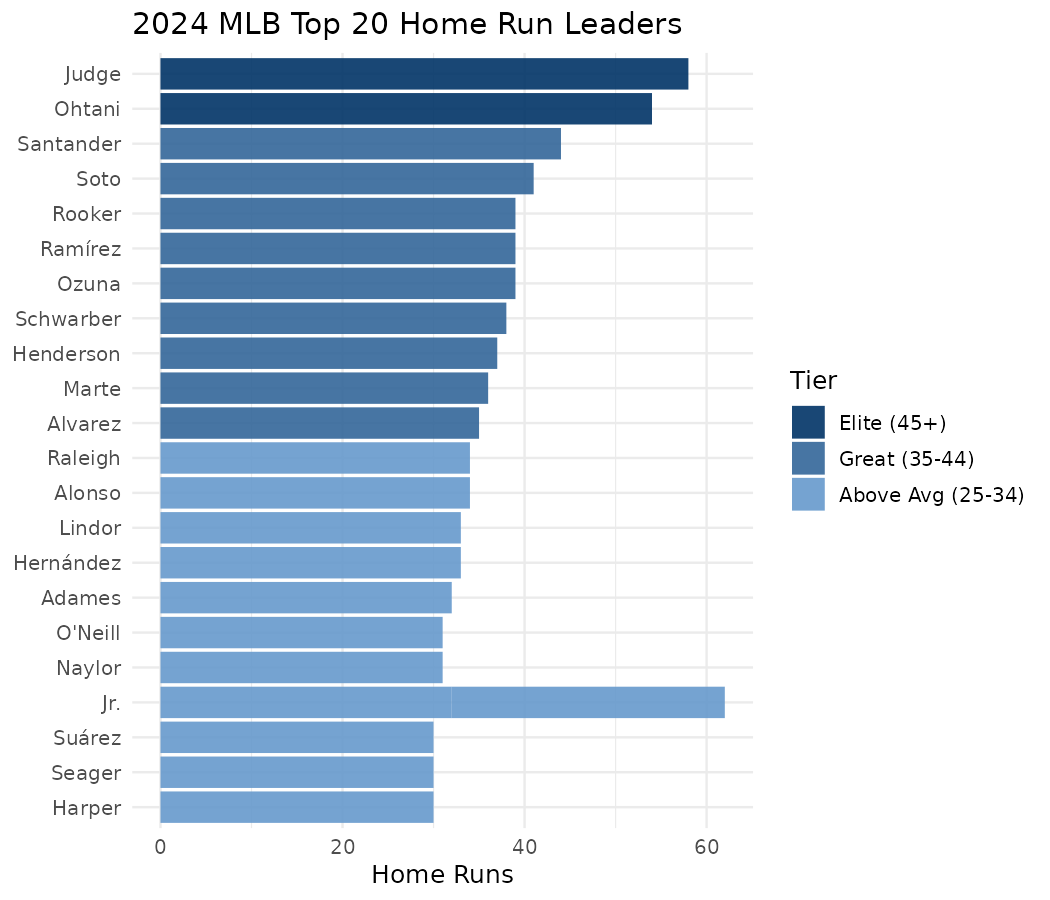
\includegraphics[width=0.78\textwidth]{PS6a_Zavala.png}
  \caption{Top 20 MLB home run leaders in 2024, colored by performance tier.}
  \label{fig:top20}
\end{figure}
 
\subsection{Distribution of Home Run Totals}
 
Figure~\ref{fig:dist} shows the distribution of home run totals across all 50 leaders. The dashed red line marks the group mean. The distribution is right-skewed, with a small number of elite hitters pulling the mean above the median.
 
\begin{figure}[h]
  \centering
  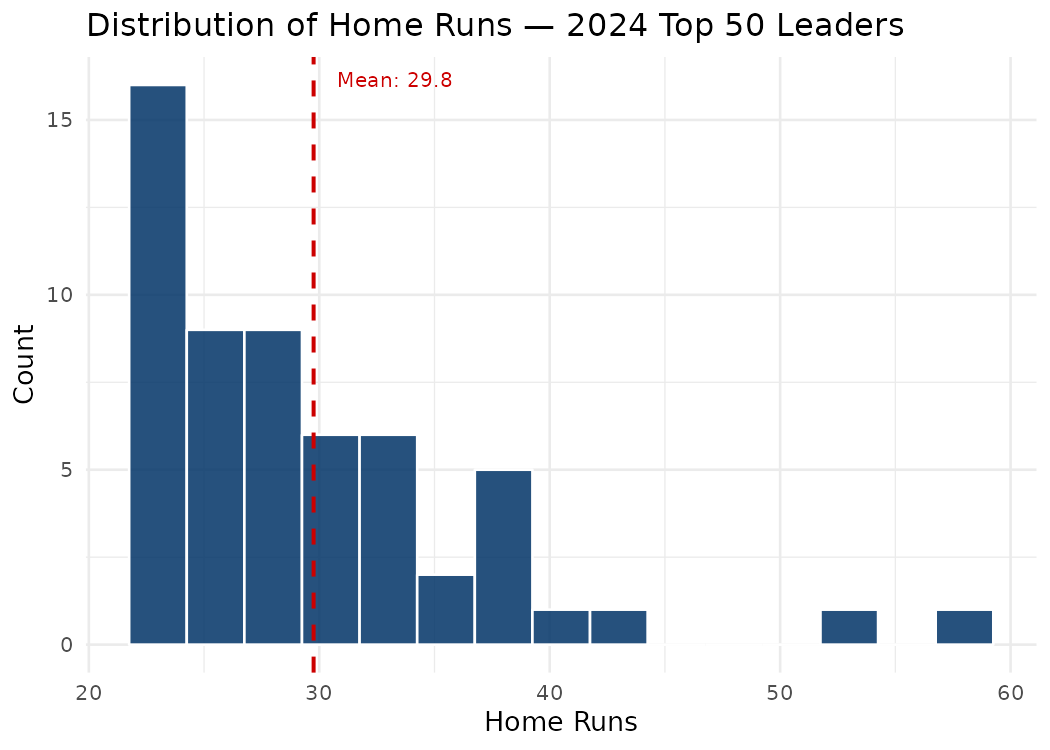
\includegraphics[width=0.78\textwidth]{PS6b_Zavala.png}
  \caption{Distribution of home run totals among the 2024 top 50 leaders.}
  \label{fig:dist}
\end{figure}
 
\subsection{Players by HR Tier}
 
Figure~\ref{fig:tier} shows the number of players falling into each HR tier. The majority of the top 50 leaders fall in the Above Average and Great tiers, with only a handful reaching the Elite threshold of 45 or more home runs.
 
\begin{figure}[h]
  \centering
  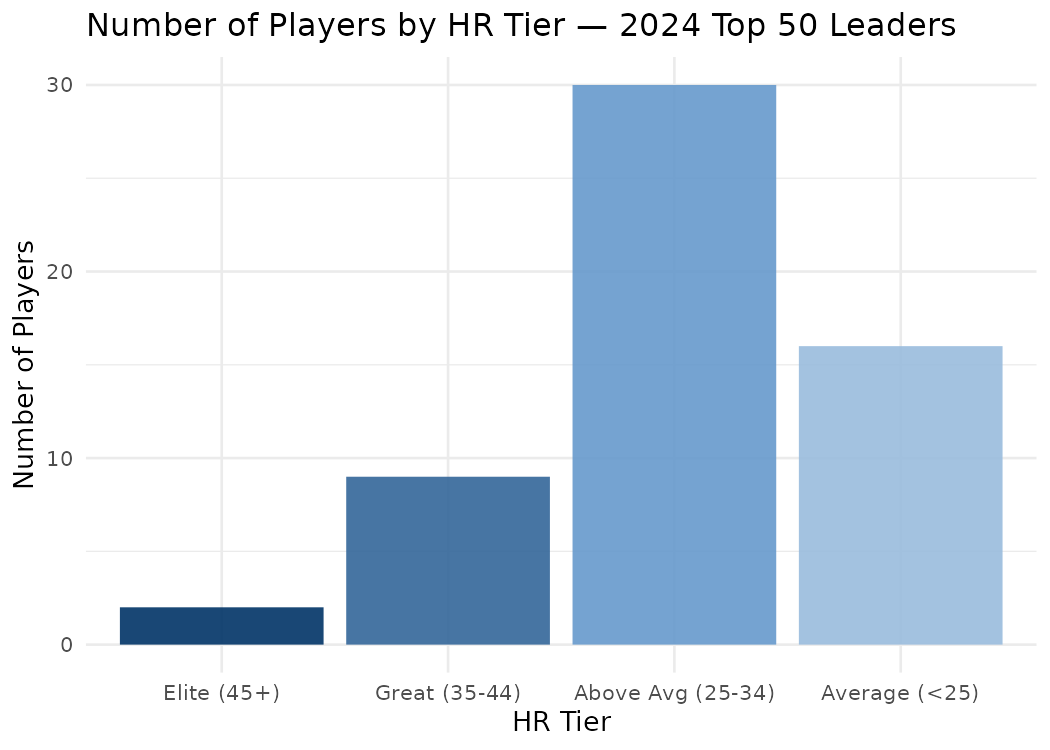
\includegraphics[width=0.78\textwidth]{PS6c_Zavala.png}
  \caption{Count of players in each HR tier among the 2024 top 50 leaders.}
  \label{fig:tier}
\end{figure}

\section{Reproducibility}
 
All steps described above are implemented in \texttt{PS6\_LastName.R}. Running that script from a fresh R session will install any missing packages, pull the data live from the MLB Stats API, perform all cleaning and transformation steps, save \texttt{mlb\_hr\_leaders\_2024\_clean.csv}, and regenerate all three figures. No manual data download is required.
 
\end{document}